\chapter{Kiegészítő modulok}
%(6 oldal): Hogyan csatlakoztak be, mit értek el, mivel lett több az egész, együttműködések menete.

% Mit adott hozzá az én témámhoz?
% Az én témámnak mely részeire tudta építeni a saját munkáját?

A mérési rendszer fejlesztése 2015 tavaszi félévében kezdődött önálló laboratóriumi munkaként. Az első működő verziót követően további témakiírások készültek hozzá kapcsolódóan. Ezek közreműködési lehetőséget biztosítottak a hallgatóknak, hogy saját munkájuk során a meglévő mérési rendszert vagy annak eredményeit felhasználják és kiegészítsék azt. A következőkben ezen munkák kerülnek bemutatásra. Az egyes leírások fontos eleme a mérési rendszerhez való hozzáadott értékek és a rendszer felhasznált szolgáltatásainak kiemelése.

Ezen együttműködéseknél rendkívül fontos volt az ismeret átadás, és a munkák koordinálása. A konzulensemmel gondot fordítottunk arra hogy minden szükséges tudást átadjunk a munkákhoz, és felügyeljük azok végrehajtását. Minden esetben elégedettek voltunk a közös munka gyümölcsével, és sokszor kellemesen meglepett milyen távolra vezettek az általunk elindított témák.

Az egyes fejezetcímek az elkészült dolgozatok címének felelnek meg.


%%%%%%%%%%%%%%%%%%%%%%%%%%%%%%%%%%%%%%%%%%%%%%%%%%%%%%%%%%%
\section{Forgalmi mérési környezet}
%Haja Dávid munkájának rövid bemutatása (2 oldal)


%%%%%%%%%%%%%%%%%%%%%%%%%%%%%%%%%%%%%%%%%%%%%%%%%%%%%%%%%%%
Haja Dávid alapszakos hallgató a szakdolgozataként választotta az általunk kiírt témát 2015 őszi félévében. Munkája során megismerte az Elméleti Áttekintés fejezet tudásanyagát, valamint a mérőrendszer felépítését. Fő tevékenységei a PlanetLab hálózat komolyabb megismerése volt, valamint a mérési rendszer kiegészítése sávszélesség kapacitás méréssel.

\subsection*{PlanetLab rendszerének megismerése}
A mérések végrehajtása során a PlanetLab hálózat gépeinek elérésével gondjaink akadtak. A tanszéken üzemelő szerverek nem megfelelően voltak felkonfigurálva, nem üzemeltek rendeltetésszerűen. A kölcsönösség elve alapján így nem fértünk hozzá a PlanetLab hálózatának szervereihez. Az említett szerverek helyre lettek állítva. 

\subsection*{D-ITG sávszélesség mérés}
A mérési rendszer eredetileg csak iperf sávszélesség mérésekkel rendelkezett, mivel ez a szoftver a legtöbb Linux alapú rendszereken, így a PlanetLab gépein is, előre telepítve volt. A mérések színvonalának érdekében az D-ITG (Distributed Internet Traffic Generator) sávszélességmérő rendszer is beépítésre került. Ez a mérőszoftver bír az elvárható alapképességekkel, mint a kinyerhető adatok széles választéka, protokoll támogatások, párhuzamos folyamok kezelése, valamint sztochasztikus adatküldő profilok is beállíthatóak. A program azonban nem elérhető a publikus csomagkezelő rendszerekből, ahonnan egyszerűen telepíthetőek lennének. Emiatt a szoftvernek egy RPM formátumú telepítőcsomagja készült el, amely megfelel a PlanetLab gépeinek rendszerének. 
Az így elkészült telepítőcsomagok automatizált telepítése az Ansible szoftverrel lett végrehajtva.

Ilyen módon új mérési lehetőségekkel bővült az eredeti rendszer. Az új mérési típus nem jöhetett volna létre a mérési rendszer rugalmassága által, a rendszer forráskódjában egyetlen osztály létrehozására volt szükség az új funkció implementálásához. Az új képességeket jól mutatja be az alábbi mérési eredmény, amely két különböző, ám hálózati szempontból közel lévő cél felé indít sávszélesség méréseket. 

\begin{figure}[!ht]
	\centering
	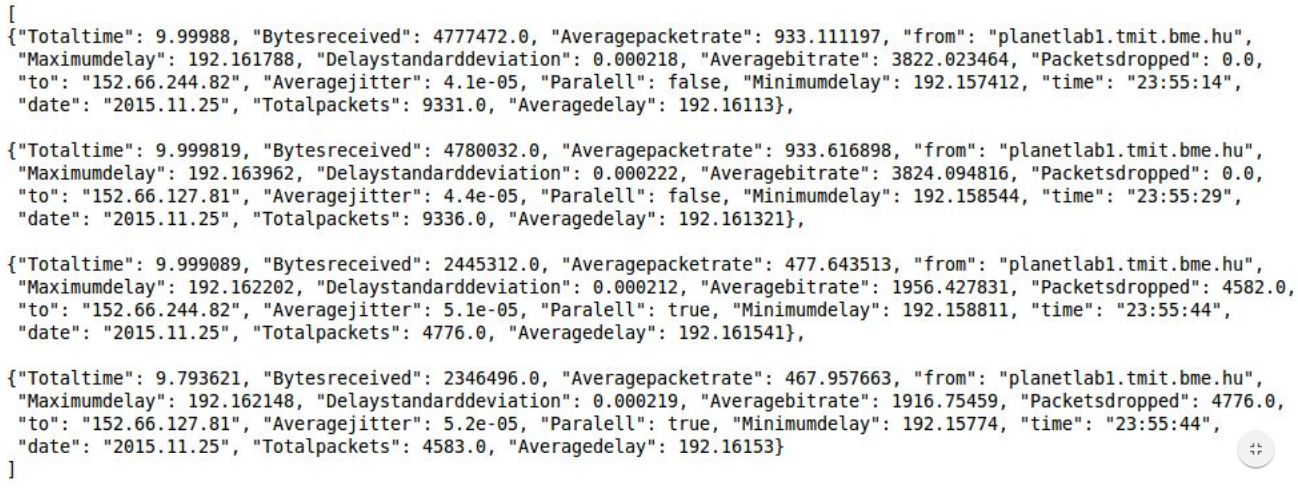
\includegraphics[width=0.95\textwidth, keepaspectratio]{figures/d-itg-measure.PNG}
	\caption{Sávszélesség mérési forgatókönyv eredménye}
	\label{fig:d-itg-measure}
\end{figure}

\newpage

A \ref{fig:d-itg-measure} ábrán látható mind a négy részeredmény ugyanahhoz a mérési forgatókönyvhöz tartozik. Alább részletezem az egyes részmérések tartalmát:

\begin{itemize}
 \setlength{\parskip}{0pt}
 \setlength{\itemsep}{0pt plus 1pt}
 
\item 10 másodperces mérés az első cél felé
\item 10 másodperces mérés a második cél felé
\item 10 másodperces mérés parallel a két cél felé, az első cél folyamának eredményeit prezentálva
\item 10 másodperces mérés parallel a két cél felé, a második cél folyamának eredményeit prezentálva
\end{itemize}


%%%%%%%%%%%%%%%%%%%%%%%%%%%%%%%%%%%%%%%%%%%%%%%%%%%%%%%%%%%
\section{AS útvonalváltozás elemzések}
%Kocsmár Bence munkájának rövid bemutatása (2 oldal)


%%%%%%%%%%%%%%%%%%%%%%%%%%%%%%%%%%%%%%%%%%%%%%%%%%%%%%%%%%%
Kocsmár Bence alapszakos hallgató szakdolgozataként választotta a mérési rendszerhez kapcsolódó témakiírást a 2016-os év tavaszi félévében. Közreműködése mutatja a legjobban a mérési rendszerben lévő potenciált, ez volt az első olyan munka amely nem a mérések végzéséhez járult hozzá, hanem a kinyert adatokat dolgozta fel. A traceroute alapú mérésekből kinyert ip útvonalak adatai lettek feldolgozva. A BGP útvonalhirdetések alapján felmért AS útvonalakkal szemben ilyen módon az útvonalakon való csomagkésleltetési idők is rendelkezésre álltak, ami többlet információkkal szolgált.

A mérési rendszer által kinyert adatok több adatfeldolgozási folyamaton mentek keresztül, melynek során külön adatstruktúrában lettek tárolva az autonóm rendszerek belső csomagtovábbítási tulajdonságai és az AS szintű csomagtovábbítási információk. Ezt a feldolgozási lépést követően az azonos forrás-cél útvonalakhoz tartozó adatok aggregálásra kerülte, hogy később historikus elemzést lehessen rajtuk végezni.

\subsection{Új AS kapcsolatok felderítése}

\begin{figure}[!ht]
	\centering
	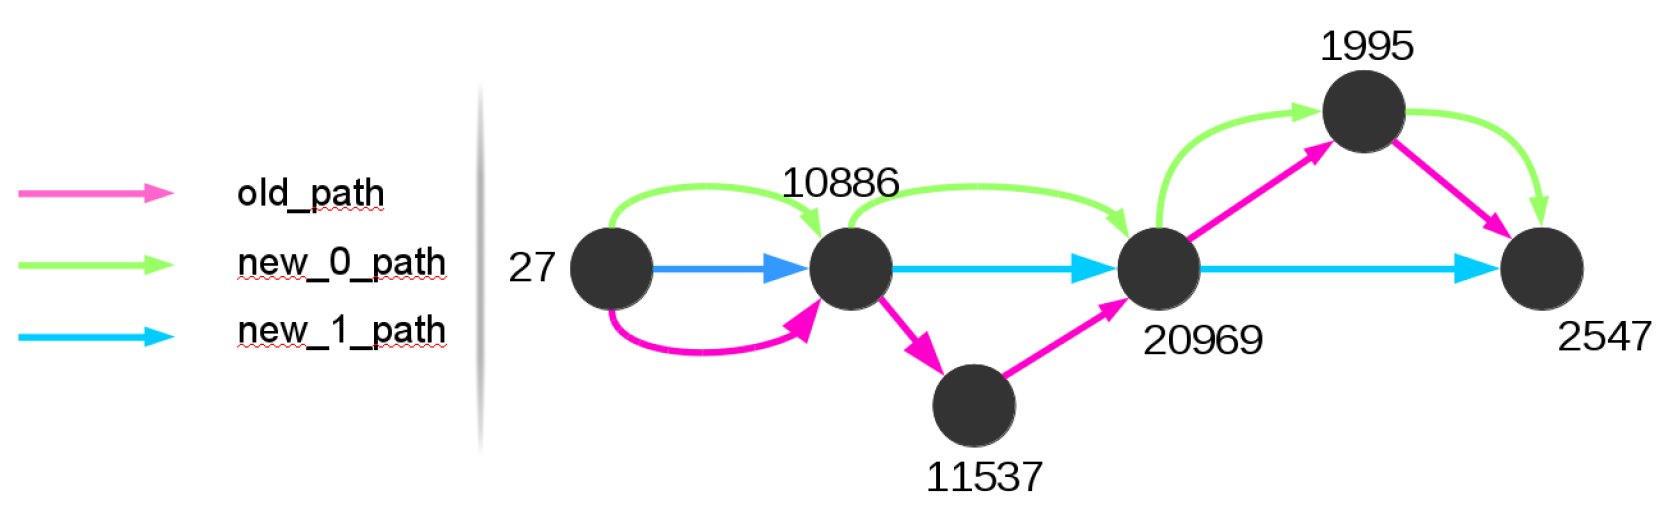
\includegraphics[width=0.70\textwidth, keepaspectratio]{figures/as-path-change-graph.PNG}
	\caption{AS-es között felderített útvonal kapcsolatok}
	\label{fig:as-path-change-graph}
\end{figure}

A kinyert AS útvonalak adatai útvonalváltozások észlelésére lettek felhasználva. A \ref{fig:as-path-change-graph} ábrán egy ilyen útvonalváltozás van reprezentálva, ahol a mérések során három különböző útvonal lett detektálva ugyanazon ip forrás és cél esetén. A lila útvonal volt legelőször használatban, majd idővel két új jött létre. Az új útvonalak mind kevesebb AS-t érintettek, ami arra a következtetésre ad okot, hogy új AS összeköttetés jött létre. A legújabb, kék útvonal, szintén rövidebb a korábbi zöldnél. Az ilyen új AS partnerkapcsolatok létrejötte mutatja a szolgáltatók igyekezetét arra, hogy minél jobb minőségű, minél rövidebb csomagtovábbítási útvonalakat építsenek ki egymás között. 

\begin{figure}[!ht]
	\centering
	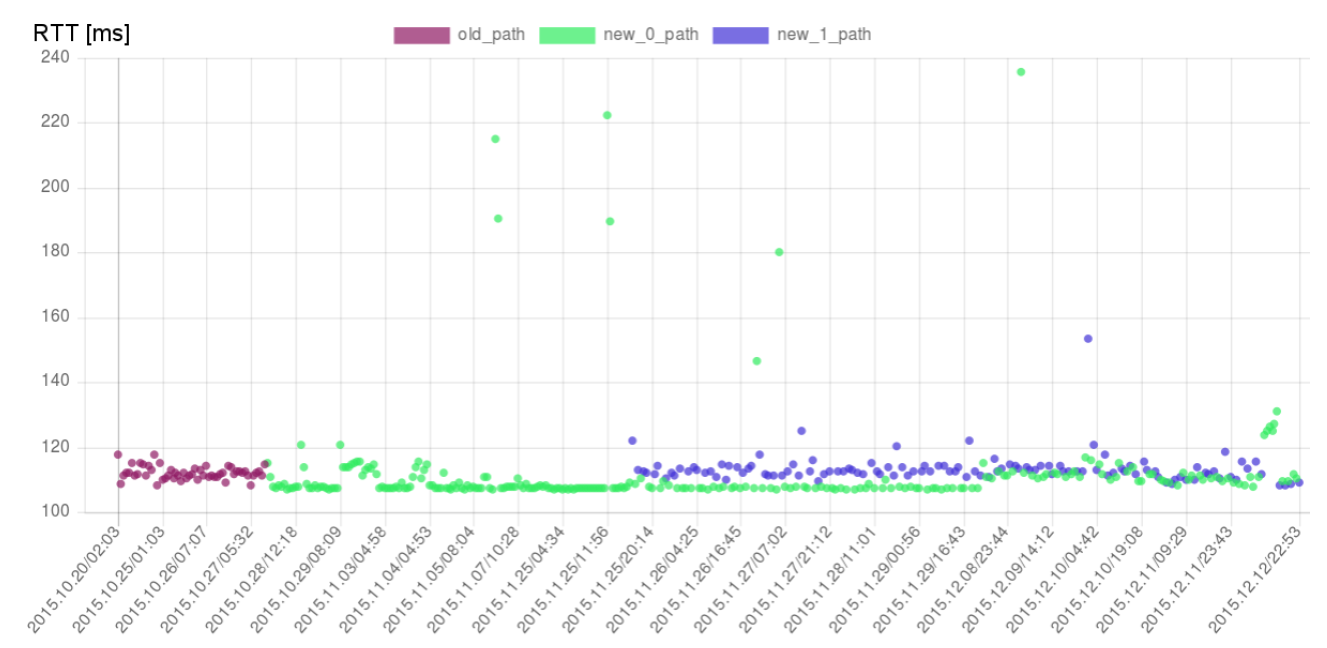
\includegraphics[width=0.95\textwidth, keepaspectratio]{figures/as-path-change-diagram.PNG}
	\caption{AS útvonalak használatának időbeli lefutása és késleltetéseik}
	\label{fig:as-path-change-diagram}
\end{figure}

A \ref{fig:as-path-change-graph} ábránál sokkal több információ olvasható le a \ref{fig:as-path-change-diagram} ábráról, amely nem csak az útvonalak időbeli feléledéseit mutatja, hanem a csomagkésleltetési tulajdonságokat. Erről leolvasható hogy az első útvonal gyakorlatilag megszűnt, ezzel szemben a két új útvonal felváltva vannak használva. Ennek oka lehet kapacitáselosztás vagy kísérleti üzem is. Ezt a sejtést megerősíti, hogy a RIPE szabadon elérhető adatbázisa\footnote{\url{https://apps.db.ripe.net/search/query.html}} alapján 2014 februárjáig nem volt összeköttetés az 10886-os s a 20965-ös AS között. A 20965-ös AS szám a GEANT szolgáltatóhoz tartozik, amely rendkívül nagy európai hálózattal és kapacitásokkal rendelkezik. A trend alapján a kisebb AS-ek igyekeznek közvetlen összeköttetést kiépíteni hozzá. A \ref{fig:as-path-change-diagram} ábráról mindezeken felül megállapítható, hogy a zöld útvonal rendkívül stabil 111 ms-os késleltetést garantált, amely kicsit gyorsabb a többinél, mindezt pedig kisebb variancia mellett.

\subsection{További útvonal információk}

A vizsgálatok fókuszában az AS útvonalváltozások álltak, azonban további tulajdonságok is kimutathatóvá váltak a mérési rendszer adatainak feldolgozásával. Erre egy említésre méltóbb példa az egyes autonóm rendszerek belső csomagtovábbítási eljárása. A \ref{fig:as-inside} ábrán a belső továbbítás során átlagosan érintett IP csomópontok száma látható az egyes AS-ek esetében.

\begin{figure}[!ht]
	\centering
	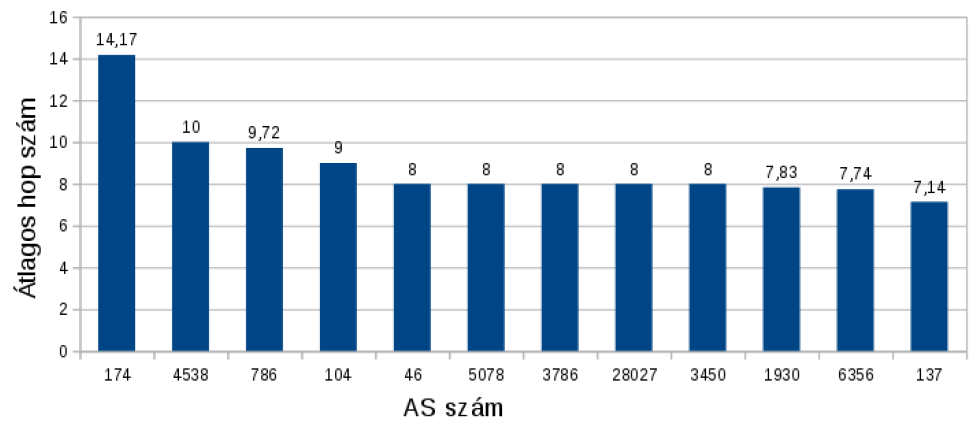
\includegraphics[width=0.9\textwidth, keepaspectratio]{figures/as-inside.PNG}
	\caption{Az autonóm rendszerek belső átlagos hop száma}
	\label{fig:as-inside}
\end{figure}

A mérések során leghosszabb belső hop számmal az amerikai Cogent tier 0-ás szolgáltató állt, átlagosan több mint 14 csomóponttal, amely a CAIDA által számított sorrend\footnote{\url{http://as-rank.caida.org/}} alapján a második legnagyobb AS. A második legtöbb hop számmal a 4538-as AS számú China Education and Research Network Center rendelkezett, amely a 1921-es a CAIDA rangsorában.


%%%%%%%%%%%%%%%%%%%%%%%%%%%%%%%%%%%%%%%%%%%%%%%%%%%%%%%%%%%
\section{Felhő alapú környezet}
%Patkó Ákos munkájának rövid bemutatása (1-2 oldal)


%%%%%%%%%%%%%%%%%%%%%%%%%%%%%%%%%%%%%%%%%%%%%%%%%%%%%%%%%%%
Patkó Ákos alapszakos hallgató önálló laboratóriumi témaként választotta a mérési rendszerhez tartozó kiírásunkat a 2016-os tavaszi félévben. A korábbi üzemeltetési problémák megoldása, valamint a könnyebb telepíthetőség és üzemeltethetőség érdekében egyéb fejlesztéseket szerepeltek a témakiírás céljaiként.

\subsection*{A mérési rendszer felhő alapú üzemeltetése}
A mérési rendszer 2015 tavaszán az egyetem egyik magánhasználatú gépén üzemelt. Ezen időszak során többször állt le a rendszer a nem megfelelő üzemeltetési környezet miatt. Ezt javítandó 2015 őszén a RedHat cég által elérhető Openshift felhős platformra költöztettük a rendszert, egy ingyenes csomagot felhasználva. A használt csomag korlátai újabb problémákat okoztak.

A mérési rendszer igényeihez illeszkedő felhős szolgáltatások össze lettek hasonlítva, amely során fel lettek mérve azok a mérésekhez kapcsolódó képességeik. A DigitalOcean cég egyik alapcsomagja felelt meg a legjobban az igényekhez.
A mérési rendszer és annak függőségeinek telepítését követően a mérési adatok könnyű elérése érdekében az adatbázishoz tartozó webes felület is telepítésre került.

\subsection*{A mérési rendszer konténerizációja}
A könnyebb telepíthetőség érdekében a Docker szoftver által támogatott konténer formátumba is be lett csomagolva a mérési rendszer. Ezt felhasználva a rendszer az összes függőségeivel együtt könnyen telepíthető és indítható.
A felhasználónak/adminisztrátornak nem szükséges manuálisan minden egyes komponenst telepíteni, felkonfigurálni és elindítani. Ezek mind egybecsomagolva telepíthetőek és elindíthatóak pár Docker paranccsal.














